\documentclass[11pt, oneside]{article} 
\usepackage{geometry}
\geometry{letterpaper} 
\usepackage{graphicx}
	
\usepackage{amssymb}
\usepackage{amsmath}
\usepackage{parskip}
\usepackage{color}
\usepackage{hyperref}

\graphicspath{{/Users/telliott_admin/Dropbox/Tex/png/}}
% \begin{center} \includegraphics [scale=0.4] {gauss3.png} \end{center}

\title{Value of pi using sine and cosine}
\date{}

\begin{document}
\maketitle
\Large

We can approximate the value of $\pi$ by squeezing it between the perimeter of an inscribed polygon, which is less than the circumference of the circle, and the perimeter of a circumscribed polygon, which is greater than the circumference of the circle.  
\begin{center} 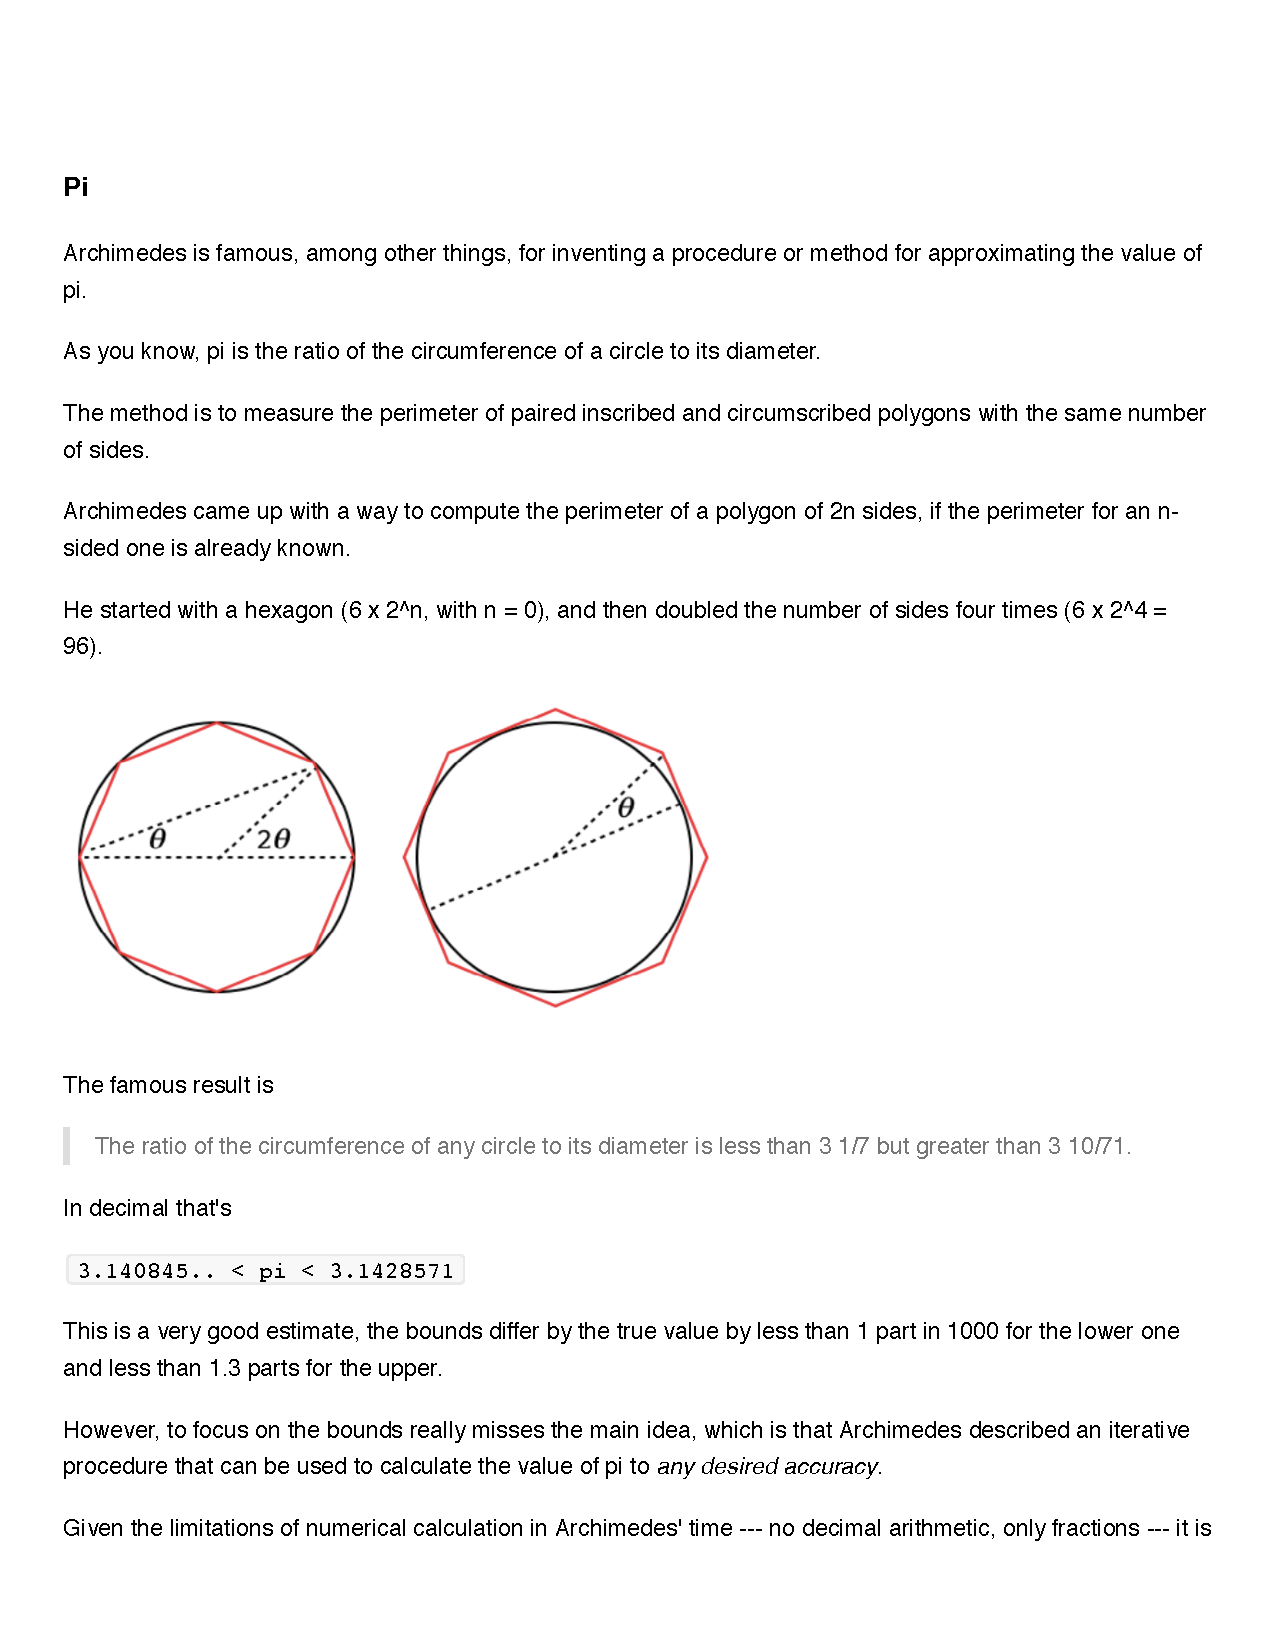
\includegraphics [scale=0.5] {pi.png} \end{center}

We use a circle of \emph{diameter} equal to $1$ (rather than the radius, which is more usual).  The circumference of the circle is then equal to $\pi$, the value which gets squeezed between the two perimeters.

The figure shows a sketch of the polygons when $n=8$.  We will be increasing the number of sides by a factor of $2$ at each step, so these are really $2^n$-gons with $n=3$ here.

\subsection*{Finding perimeters in terms of angle $\theta$}
For the left panel, we have $8$ sides, so the central angle (marked $2\theta$) is equal to
\[  \frac{2 \pi}{8} = \frac{\pi}{4} = 45^\circ \]
and $\theta$ is one-half that.  

\begin{center} \includegraphics [scale=0.3] {piL.png} \end{center}
By a standard theorem (from Thales), the triangle above containing angle $\theta$, with the diameter as one side, and two other vertices also on the circle, is a right triangle.  The inscribed n-gon side of length $S$ (shown in red) is equal to $\sin \theta$, since the hypotenuse of the triangle is the diameter of the circle, which is equal to $1$.  

The total perimeter is $8 \cdot S$.

[Alternatively, use half the angle at the center of the circle (i.e. $\theta$).  Then half the length of the red line $S/2$, divided by the radius ($r = 1/2$) gives $S = \sin \theta$, the same result.]

For the right panel, we have the same circle (now showing the outside polygon, circumscribing the circle), it is just rotated slightly..  One dashed line extends a bit further to the vertex of the n-gon outside.  The angle marked $\theta$ is one-half the angle we marked as $2 \theta$ previously since now the diameter comes down to the middle of the side.

We compute the whole length of the side $T$ as follows.  The half-side is $T/2$ and the hypotenuse of the triangle is one-half the unit diameter, which is $1/2$, so $T = \tan \theta$.  The total perimeter is $8 \cdot T$.

\begin{center} \includegraphics [scale=0.3] {piR.png} \end{center}
All of this gives us two simple equations for the two perimeters.  At each stage there are $2^n$ sides, the length of each short side $S$ on the inside equals $\sin \theta$ and the length of each short side on the outside $T$ is equal to $\tan \theta$, where $\theta = 2 \pi/2^n$.

The total length of the inside perimeter is $nS = n \sin \theta$ and that of the outside is $nT = n \tan \theta$.  When we go from $\theta$ to $\theta/2$ and $n$ to $2n$, we must compute the new values $S'$ and $T'$ from $S$ and $T$ using the half-angle formulas, and then also multiply by 2 to take account of the change from $n$ to $2n$ for the total circumference.

\subsection*{Base case:  square}
If we go back to the square ($n=2, 2^n = 4$), then the angle $\theta$ is $\pi/4$.

The tangent is $T = \tan \pi/4 = 1$ and the sine is $S = \sin \pi/4 = 1/\sqrt{2}$.  

Our formulas say that on the inside, the perimeter is $4S = 4/\sqrt{2} = 2 \sqrt{2}$ and on the outside, the perimeter is $4T = 4$.  

From simple geometry, we can calculate that the circumscribing square has a side length which is twice the radius of the circle, that is, $1$ for our  circle with unit diameter, so its perimeter is $4$, which checks.

\begin{center} \includegraphics [scale=0.4] {square_perimeter.png} \end{center}

Similarly, an inscribed square can be decomposed into four isosceles right triangles with sides of length $1/2$ and hypotenuse $1/\sqrt{2}$, so the total perimeter is $4/\sqrt{2}$, which also checks.

Now, what we are going to do is to increase $n$ in steps of 1, that increases $2^n$ by a factor of $2^1 = 2$ each time.  Doubling $n$ halves the angle.  So all we need is a way to compute trigonometric functions of $\theta/2$, knowing the values for $\theta$, so we can calculate what happens to the perimeter.  We already know how to do that.

\subsection*{Half angle formulas}

We have derived these elsewhere.  Refer to this \hyperref[sec:double_half_angles]{\textbf{chapter}}.

The unprimed values refer to angle $\theta$, while the primed ones have angle $\theta/2$.

\[ C' = \sqrt{\frac{1}{2} (1 + C)}  \]
This can be rearranged (e.g.) to give $2[C']^2 = 1 + C$, which we'll use in a second.

\[ S' = \frac{S}{2 C'} \]

\[ T' = \frac{S'}{C'} = \frac{S}{2 [C']^2} \]
\[  = \frac{S}{1 + C} \]

So, given $S, C$ and $T$, first calculate $C'$ and $T'$ and then $S'$.  

To get the perimeters, remember that factor of two from doubling $n$, the number of sides.  The inside perimeter is the sine $S'$ and the outside perimeter is the tangent $T'$.

\subsection*{Calculation}

Above we have for the square that the angle is $45$ degrees or $\pi/4$ and the inside (p) and outside (P) perimeters are:

$\bullet$  $p = 4/\sqrt{2}$

$\bullet$  $P = 4$

Also, the $\sin \theta = \cos \theta = 1/\sqrt{2}$ while $\tan \theta = 1$.

\subsection*{one round}
\[ C' = \sqrt{\frac{1}{2} (1 + C)} = \sqrt{\frac{1}{2} (1 + \frac{1}{\sqrt{2}} )} = 0.92387953 \]

This checks out as equal to $\cos \pi/8$.
\[ S' = \frac{S}{2 C'} = 0.38268343 \]
\[ T' = \frac{S'}{C'} = 0.41421356 \]
Then
\[ p = 8 S' = 3.06146744 \]
\[ P = 8 T' = 3.31370848 \]

I wrote a script to do this:

\url{https://gist.github.com/telliott99/433a73eb708e25a1d6f6ba5291f48ebf}

Output:

\begin{verbatim}
> python script.py 
round 1
4
2.82842712475
4.0

round 2
8
3.06146745892
3.31370849898

round 3
16
3.12144515226
3.18259787807

...

round 15
65536
3.14159265239
3.141592656

3.14159265359
> 

\end{verbatim}

\end{document}